\documentclass[preprint,12pt,aps,pra,showkeys,amsmath,amssymb,superscriptaddress,floatfix]{revtex4-2}
\usepackage[T1]{fontenc}
\usepackage[utf8]{inputenc}
\usepackage{amsmath,amssymb,amsthm,mathtools,mathrsfs}
\usepackage{microtype,booktabs,enumitem}
\usepackage{xcolor,tikz,etoolbox}
\usepackage[skins,breakable]{tcolorbox}
\usepackage{needspace}
% Keep diagram geometry independent of REVTeX preprint body spacing.
\AtBeginEnvironment{tikzpicture}{\linespread{1}\selectfont}
\usetikzlibrary{arrows.meta,positioning,calc,fit,decorations.pathreplacing}
\usepackage{graphicx}
\usepackage{hyperref}

\definecolor{MMBlue}{RGB}{0,82,155}
\definecolor{MMOrange}{RGB}{200,80,0}
\tikzset{
 mmnode/.style={draw=MMBlue,rounded corners=2pt,fill=MMBlue!4,align=left,execute at begin node={\raggedright},text width=5cm,font=\fontsize{10}{12}\selectfont,inner sep=6pt},
 mmimport/.style={mmnode,draw=black!65,fill=black!4},
 mmcandidate/.style={mmnode,draw=MMOrange,dashed,fill=MMOrange!5},
 mmrejected/.style={mmnode,draw=black,densely dotted,fill=black!8},
 mmproof/.style={->,thick,MMBlue},
 mmflow/.style={->,semithick,black!70},
 mmrepair/.style={->,dashed,thick,MMOrange},
 mmcandidatearrow/.style={->,dashed,semithick,MMOrange},
 mmnote/.style={font=\scriptsize,fill=white,inner sep=2pt,align=center}}

\usepackage[section]{placeins}
\setlength{\emergencystretch}{3em}
\setlist{itemsep=3pt,topsep=4pt}
\newtheorem{theorem}{Theorem}[section]
\newtheorem{proposition}[theorem]{Proposition}
\newtheorem{lemma}[theorem]{Lemma}
\newtheorem{corollary}[theorem]{Corollary}
\theoremstyle{definition}
\newtheorem{definition}[theorem]{Definition}
\newtheorem{example}[theorem]{Example}
\theoremstyle{remark}
\newtheorem{remark}[theorem]{Remark}
% Avoid isolated statement headings and single-line paragraph fragments.
\BeforeBeginEnvironment{theorem}{\Needspace{6\baselineskip}}
\BeforeBeginEnvironment{definition}{\Needspace{5\baselineskip}}
\BeforeBeginEnvironment{proposition}{\Needspace{5\baselineskip}}
\BeforeBeginEnvironment{lemma}{\Needspace{5\baselineskip}}
\BeforeBeginEnvironment{corollary}{\Needspace{5\baselineskip}}
\clubpenalty=5000
\widowpenalty=5000
\newcommand{\R}{\mathbb R}\newcommand{\Z}{\mathbb Z}\newcommand{\N}{\mathbb N}
\newcommand{\Pa}{\operatorname{Pa}}\newcommand{\Desc}{\operatorname{Desc}}
\newcommand{\cl}{\operatorname{cl}}\newcommand{\cost}{\operatorname{cost}}
\newcommand{\status}{\operatorname{status}}
% Faculty cards: a visual rail groups the five faculties within one agent.
% The rail has no arrowhead and does not represent a proof dependency.
\newcommand{\mmfacultybadge}[1]{%
 \node[circle,draw=MMBlue,line width=1pt,fill=white,
 minimum size=7mm,inner sep=0pt,font=\sffamily\small\bfseries,text=MMBlue]
 at ([xshift=15pt,yshift=-15pt]frame.north west) {#1};}
\newcommand{\mmfacultyrail}{%
 \draw[MMBlue!80,line width=1pt]
 ([xshift=15pt,yshift=2pt]frame.north west)--
 ([xshift=15pt,yshift=-2pt]frame.south west);}
\newtcolorbox{mmfacultybox}[2]{enhanced,breakable,
 colback=MMBlue!4,colframe=MMBlue!4,boxrule=0pt,arc=3pt,
 left=39pt,right=9pt,top=4pt,bottom=4pt,
 before skip=2pt,after skip=2pt,
 fontupper=\small\linespread{1.1}\selectfont,
 overlay unbroken={\mmfacultyrail\mmfacultybadge{#1}},
 overlay first={\mmfacultyrail\mmfacultybadge{#1}},
 overlay middle={\mmfacultyrail},overlay last={\mmfacultyrail}}
\newcommand{\mmfaculty}[3]{%
 \begin{mmfacultybox}{#1}{#2}
 {\sffamily\bfseries\color{MMBlue}#2}\par\smallskip #3
 \end{mmfacultybox}}
\newcommand{\agent}[9]{%
 \Needspace{8\baselineskip}
 \subsubsection{#1}
 \noindent\textbf{Object.} #2\par
 \noindent\textbf{Role.} #3\par\smallskip
 \mmfaculty{E}{Ego}{#4}
 \mmfaculty{M}{Memory}{#5}
 \mmfaculty{I}{Intellect}{#6}
 \mmfaculty{S}{Sense}{#7}
 \mmfaculty{A}{Action}{#8}
 \smallskip\noindent #9\par}

\usepackage{longtable,array,calc}
\providecommand{\tightlist}{\setlength{\itemsep}{2pt}\setlength{\parskip}{0pt}}
\makeatletter
\def\frontmatter@abstract@produce{\par\addvspace{\frontmatter@preabstractspace}%
\begingroup\prep@absbox\unvbox\absbox\post@absbox\endgroup
\addvspace{\frontmatter@postabstractspace}}
\makeatother
\newcommand{\field}[2]{\par\smallskip\noindent\textbf{#1.} #2\par}
\setlength{\emergencystretch}{5em}
\AtBeginEnvironment{verbatim}{\small\linespread{1.0}\selectfont}


\hypersetup{colorlinks=true,linkcolor=MMBlue,urlcolor=MMBlue,pdfauthor={Dibakar Sigdel}}

\begin{document}

\title{Hilbert Basis Theorem and Affine Finiteness\\[4pt]\large An End-to-End Meta-Math Walkthrough}

\author{Dibakar Sigdel}

\affiliation{Mindverse Computing LLC, Lynnwood, WA 98087, USA}

\date{October 2026}

\begin{abstract}

Collect possible coefficients at each degree into an ascending chain of
ideals. Once that chain stabilizes, finitely many chosen polynomials
reduce every other polynomial by decreasing degree. The report presents
the target theorem, declared imports, a dependency graph, five-faculty
node contracts, a continuous proof, a worked example, and a
hypothesis-repair audit. It is an authored mathematical exposition, not
a deployed-agent transcript or a formal proof-assistant certificate.

\end{abstract}\maketitle\linespread{1.12}\selectfont

\noindent\textbf{AG-01 / Algebraic Geometry / Report v1}

\section{Target and import contract}

\begin{theorem}

If \(R\) is a commutative Noetherian ring with identity (every ideal is
finitely generated), then \(R[x]\) is Noetherian. Deduce by induction
that every ideal of \(k[x_1,\ldots,x_n]\) is finitely generated for a
field \(k\), so every affine algebraic set is cut out by finitely many
polynomial equations.

\end{theorem}

\subsection{Foundations and permitted imports}

Use elementary ideal arithmetic and polynomial coefficients, including
degree reduction by cancellation of a leading coefficient. Noetherianity
implies the ascending chain condition: the union of an ascending chain
is an ideal; its finitely many generators all lie in one term, which
therefore equals the union. For an ideal \(I\), \(V(I)\) denotes its
common zero set over the chosen field. No algebraic closure hypothesis
is needed here.

\clearpage\section{Node interaction workflow}

\begin{center}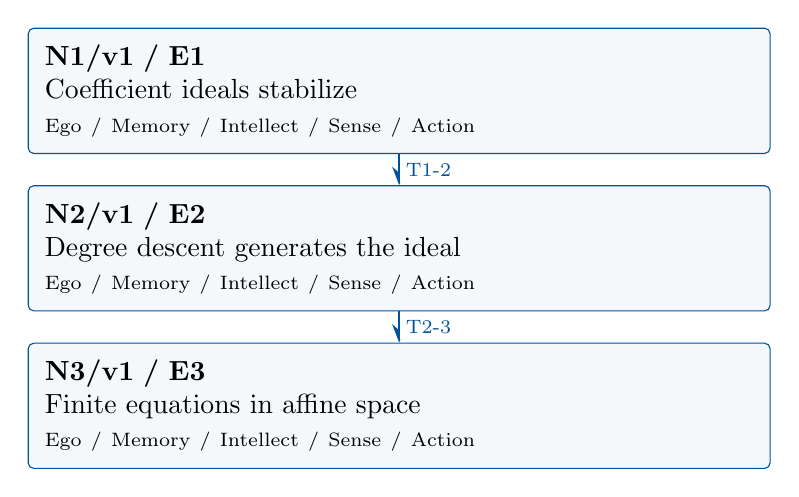
\begin{tikzpicture}[>=Stealth,x=1cm,y=1cm]

\node[mmnode,text width=9cm,minimum height=1.25cm] (N1) at (0,0.0) {\textbf{N1/v1 / E1}\\Coefficient ideals stabilize\\{\scriptsize Ego / Memory / Intellect / Sense / Action}};

\node[mmnode,text width=9cm,minimum height=1.25cm] (N2) at (0,-2.0) {\textbf{N2/v1 / E2}\\Degree descent generates the ideal\\{\scriptsize Ego / Memory / Intellect / Sense / Action}};

\node[mmnode,text width=9cm,minimum height=1.25cm] (N3) at (0,-4.0) {\textbf{N3/v1 / E3}\\Finite equations in affine space\\{\scriptsize Ego / Memory / Intellect / Sense / Action}};

\draw[mmproof] (N1.south) -- node[mmnote,right] {T1-2} (N2.north);

\draw[mmproof] (N2.south) -- node[mmnote,right] {T2-3} (N3.north);

\end{tikzpicture}\end{center}

Each box is one mathematical agent containing all five faculties. Blue
arrows carry the versioned exports listed below. The layout gives a
reading order; only drawn arrows assert dependencies. Diagnostic repair
is separate from the proof DAG.

\subsection{Versioned evidence-transfer ledger}

\begingroup\small\linespread{1.05}\selectfont

\Needspace{5\baselineskip}\field{T1-2: N1/E1/v1 to N2}{There is \(N\) with \(A_d=A_N\) for all \(d\ge N\), and each \(A_d\) for
\(d\le N\) has finitely many chosen polynomial lifts in \(I\).}

\field{Receiving activity}{N2.1}

\field{Compatibility}{E1/v1 and the ideal \(J\) generated in \(R[x]\) by the finite chosen
family. Check: The degree must strictly decrease after cancellation,
even when \(R\) has zero divisors.}

\Needspace{5\baselineskip}\field{T2-3: N2/E2/v1 to N3}{\(I=J\), so \(R[x]\) is Noetherian.}

\field{Receiving activity}{N3.1}

\field{Compatibility}{E2/v1 and a field \(k\), whose only ideals are \(0\) and \(k\). Check:
Equality of zero sets follows from linear combinations of equations, not
from radical-ideal correspondence.}

\endgroup

\clearpage\section{Agent roles and five-faculty activities}\begingroup\small\linespread{1.05}\selectfont\setlist{itemsep=1pt,topsep=2pt}

\subsection{N1/v1: Coefficient ideals stabilize}

\field{Object and role}{Encode infinitely many polynomial constraints in an ascending chain
inside the Noetherian coefficient ring. \textbf{Local obligation:} There
is \(N\) with \(A_d=A_N\) for all \(d\ge N\), and each \(A_d\) for
\(d\le N\) has finitely many chosen polynomial lifts in \(I\).}

\field{Inputs}{An ideal \(I\subset R[x]\) and
\(A_d=\{\text{coefficient of }x^d\text{ in }f:f\in I,\deg f\le d\}\),
including zero.}

\mmfaculty{E}{Ego}{Publish E1/v1 only after establishing this obligation: There is \(N\)
with \(A_d=A_N\) for all \(d\ge N\), and each \(A_d\) for \(d\le N\) has
finitely many chosen polynomial lifts in \(I\).}

\mmfaculty{M}{Memory}{An ideal \(I\subset R[x]\) and
\(A_d=\{\text{coefficient of }x^d\text{ in }f:f\in I,\deg f\le d\}\),
including zero. Retain the stated assumptions and import versions.}

\mmfaculty{I}{Intellect}{Encode infinitely many polynomial constraints in an ascending chain
inside the Noetherian coefficient ring.}

\mmfaculty{S}{Sense}{Use coefficient ideals at degree at most \(d\); a set of leading
coefficients at exactly one degree requires care under cancellation.}

\mmfaculty{A}{Action}{Carry out activities N1.1--N1.2 below, retaining each calculation and
construction as evidence.}

\smallskip\noindent\textbf{Numbered mathematical activities}

\begin{enumerate}[label=N1.\arabic*,leftmargin=3.4em]

\item Addition and scalar multiplication of polynomials of degree at most
\(d\) show that \(A_d\) is an ideal of \(R\). Multiplication by \(x\)
shows \(A_d\subset A_{d+1}\). The ascending chain condition gives
stabilization at some \(N\).

\item For \(0\le d\le N\), choose generators \(a_{d,1},\ldots,a_{d,r_d}\) of
\(A_d\). Omit zero generators. Choose \(f_{d,j}\in I\) of degree at most
\(d\) whose coefficient at \(x^d\) is \(a_{d,j}\). A nonzero chosen
coefficient makes its degree exactly \(d\). There are only finitely many
chosen polynomials.

\end{enumerate}

\field{Export E1/v1}{There is \(N\) with \(A_d=A_N\) for all \(d\ge N\), and each \(A_d\) for
\(d\le N\) has finitely many chosen polynomial lifts in \(I\).}

\field{Acceptance gate}{Use coefficient ideals at degree at most \(d\); a set of leading
coefficients at exactly one degree requires care under cancellation.}

\field{Targeted repair}{If a sum cancels leading coefficients, retain the coefficient-at-degree
definition, which includes zero and remains an ideal. Withhold this
export and recheck its descendants after a versioned correction.}

\clearpage

\subsection{N2/v1: Degree descent generates the ideal}

\field{Object and role}{Cancel the highest coefficient of an arbitrary polynomial in \(I\) and
use induction on its degree. \textbf{Local obligation:} \(I=J\), so
\(R[x]\) is Noetherian.}

\field{Inputs}{E1/v1 and the ideal \(J\) generated in \(R[x]\) by the finite chosen
family. Incoming proof exports: E1/v1 at N2.1.}

\mmfaculty{E}{Ego}{Publish E2/v1 only after establishing this obligation: \(I=J\), so
\(R[x]\) is Noetherian.}

\mmfaculty{M}{Memory}{E1/v1 and the ideal \(J\) generated in \(R[x]\) by the finite chosen
family. Incoming proof exports: E1/v1 at N2.1. Retain the stated
assumptions and import versions.}

\mmfaculty{I}{Intellect}{Cancel the highest coefficient of an arbitrary polynomial in \(I\) and
use induction on its degree.}

\mmfaculty{S}{Sense}{The degree must strictly decrease after cancellation, even when \(R\)
has zero divisors.}

\mmfaculty{A}{Action}{Carry out activities N2.1--N2.2 below, retaining each calculation and
construction as evidence.}

\smallskip\noindent\textbf{Numbered mathematical activities}

\begin{enumerate}[label=N2.\arabic*,leftmargin=3.4em]

\item Certainly \(J\subset I\). Let nonzero \(f\in I\) have degree \(m\) and
leading coefficient \(a\). Set \(d=\min(m,N)\). Stabilization gives
\(a\in A_m=A_d\) when \(m>N\), and membership is immediate when
\(m\le N\). Write \(a=\sum_j b_j a_{d,j}\) with \(b_j\in R\).

\item The polynomial \(h=f-\sum_j b_j x^{m-d}f_{d,j}\) lies in \(I\) and has
degree less than \(m\) or is zero. Strong induction on the nonnegative
integer \(m\) proves \(h\in J\), hence \(f\in J\). At \(m=0\),
cancellation leaves zero, which starts the induction. No division by a
leading coefficient was used.

\end{enumerate}

\field{Export E2/v1}{\(I=J\), so \(R[x]\) is Noetherian.}

\field{Acceptance gate}{The degree must strictly decrease after cancellation, even when \(R\)
has zero divisors.}

\field{Targeted repair}{If polynomial long division over a field is used for a general ring,
replace it by the generator combination above; invertibility is not
assumed. Withhold this export and recheck its descendants after a
versioned correction.}

\clearpage

\subsection{N3/v1: Finite equations in affine space}

\field{Object and role}{Iterate the one-variable theorem and translate ideal generation into
equality of zero sets. \textbf{Local obligation:} Every
\(I\subset k[x_1,\ldots,x_n]\) has finite generators \(g_1,\ldots,g_s\)
and \(V(I)=V(g_1,\ldots,g_s)\).}

\field{Inputs}{E2/v1 and a field \(k\), whose only ideals are \(0\) and \(k\). Incoming
proof exports: E2/v1 at N3.1.}

\mmfaculty{E}{Ego}{Publish E3/v1 only after establishing this obligation: Every
\(I\subset k[x_1,\ldots,x_n]\) has finite generators \(g_1,\ldots,g_s\)
and \(V(I)=V(g_1,\ldots,g_s)\).}

\mmfaculty{M}{Memory}{E2/v1 and a field \(k\), whose only ideals are \(0\) and \(k\). Incoming
proof exports: E2/v1 at N3.1. Retain the stated assumptions and import
versions.}

\mmfaculty{I}{Intellect}{Iterate the one-variable theorem and translate ideal generation into
equality of zero sets.}

\mmfaculty{S}{Sense}{Equality of zero sets follows from linear combinations of equations, not
from radical-ideal correspondence.}

\mmfaculty{A}{Action}{Carry out activities N3.1--N3.2 below, retaining each calculation and
construction as evidence.}

\smallskip\noindent\textbf{Numbered mathematical activities}

\begin{enumerate}[label=N3.\arabic*,leftmargin=3.4em]

\item A field is Noetherian. Apply E2 successively to \(k\), \(k[x_1]\), and
so on to obtain Noetherianity of \(k[x_1,\ldots,x_n]\). The induction
length is the finite number of variables.

\item If \(I=(g_1,\ldots,g_s)\), a point annihilating all generators
annihilates each finite polynomial combination of them, hence all of
\(I\). The reverse implication is immediate because the generators
belong to \(I\). This proves the finite-equation conclusion.

\end{enumerate}

\field{Export E3/v1}{Every \(I\subset k[x_1,\ldots,x_n]\) has finite generators
\(g_1,\ldots,g_s\) and \(V(I)=V(g_1,\ldots,g_s)\).}

\field{Acceptance gate}{Equality of zero sets follows from linear combinations of equations, not
from radical-ideal correspondence.}

\field{Targeted repair}{If finite generation is claimed for infinitely many variables, restore
the finite-variable contract before reusing the induction. Withhold this
export and recheck its descendants after a versioned correction.}

\endgroup\clearpage\section{Continuous mathematical proof}\label{sec:proof}

\subsection{N1 --- Coefficient ideals
stabilize}\label{n1-coefficient-ideals-stabilize}

\begin{enumerate}
\def\labelenumi{\arabic{enumi}.}
\item
  \textbf{N1.1.} Addition and scalar multiplication of polynomials of
  degree at most \(d\) show that \(A_d\) is an ideal of \(R\).
  Multiplication by \(x\) shows \(A_d\subset A_{d+1}\). The ascending
  chain condition gives stabilization at some \(N\).
\item
  \textbf{N1.2.} For \(0\le d\le N\), choose generators
  \(a_{d,1},\ldots,a_{d,r_d}\) of \(A_d\). Omit zero generators. Choose
  \(f_{d,j}\in I\) of degree at most \(d\) whose coefficient at \(x^d\)
  is \(a_{d,j}\). A nonzero chosen coefficient makes its degree exactly
  \(d\). There are only finitely many chosen polynomials.
\end{enumerate}

\subsection{N2 --- Degree descent generates the
ideal}\label{n2-degree-descent-generates-the-ideal}

\begin{enumerate}
\def\labelenumi{\arabic{enumi}.}
\item
  \textbf{N2.1.} Certainly \(J\subset I\). Let nonzero \(f\in I\) have
  degree \(m\) and leading coefficient \(a\). Set \(d=\min(m,N)\).
  Stabilization gives \(a\in A_m=A_d\) when \(m>N\), and membership is
  immediate when \(m\le N\). Write \(a=\sum_j b_j a_{d,j}\) with
  \(b_j\in R\).
\item
  \textbf{N2.2.} The polynomial \(h=f-\sum_j b_j x^{m-d}f_{d,j}\) lies
  in \(I\) and has degree less than \(m\) or is zero. Strong induction
  on the nonnegative integer \(m\) proves \(h\in J\), hence \(f\in J\).
  At \(m=0\), cancellation leaves zero, which starts the induction. No
  division by a leading coefficient was used.
\end{enumerate}

\subsection{N3 --- Finite equations in affine
space}\label{n3-finite-equations-in-affine-space}

\begin{enumerate}
\def\labelenumi{\arabic{enumi}.}
\item
  \textbf{N3.1.} A field is Noetherian. Apply E2 successively to \(k\),
  \(k[x_1]\), and so on to obtain Noetherianity of
  \(k[x_1,\ldots,x_n]\). The induction length is the finite number of
  variables.
\item
  \textbf{N3.2.} If \(I=(g_1,\ldots,g_s)\), a point annihilating all
  generators annihilates each finite polynomial combination of them,
  hence all of \(I\). The reverse implication is immediate because the
  generators belong to \(I\). This proves the finite-equation
  conclusion.
\end{enumerate}

\hfill$\square$

\section{Worked orchestration}

In \(k[x,y]\), let \(I\) be generated by \(x^2,xy,xy^2,xy^3,\ldots\).
Since \(xy^m=y^{m-1}(xy)\) for \(m\ge1\), \(I=(x^2,xy)\). Its common
zeros satisfy \(x=0\), hence \(V(I)\) is the \(y\)-axis. Finite
generation does not say \(I\) is radical: \(x\) vanishes on that axis
but \(x\notin I\).

\subsection{Boundary and hypothesis audit}

The ring \(k[x_1,x_2,\ldots]\) is not Noetherian. If the ideal
\((x_1,x_2,\ldots)\) had finitely many generators, they would involve
only finitely many variables. Setting those variables to zero would
annihilate every proposed generator but leave a later variable nonzero,
contradicting generation.

\section{Illustrative failure and repair}

The following is an authored diagnostic scenario. Changed assumptions
define a new contract; they do not retroactively prove the original
statement.

\subsection{Rejected argument, diagnosis, and correction}
\textbf{Rejected N2 activity:} divide by the leading coefficient of a
polynomial over \(R\). In \(\mathbb Z[x]\), the coefficient \(2\) need
not be invertible. \textbf{Diagnosis:} Intellect substituted a field
division algorithm for a ring argument. \textbf{Repair:} express the
leading coefficient in the ideal generated by the \(a_{d,j}\) and
subtract the corresponding polynomial combination. The degree falls
without division; recheck E2 and the affine consequence. The theorem
remains unchanged.

\subsection{Publication and reuse}
The corrected export retains its explicit assumptions. A hypothetical
revision receives a new version, and each consuming activity is
rechecked; this scenario is not a recorded runtime event. \textbf{Next
direction:} Use finite polynomial descriptions as input to elimination
and local computations; finite generation alone gives no practical
degree bound.

\par\medskip\begingroup\small\linespread{1.0}\selectfont\noindent\textbf{Provenance.} This authored proof is complete relative to its declared imports. Reuse
each export with its assumptions, proof, and version. The original
Markdown remains available for comparison.
\par\endgroup

\par\smallskip\begingroup\small\linespread{1.0}\selectfont\noindent\textbf{Further reading.} \href{https://www.jmilne.org/math/CourseNotes/ag.html}{J. S. Milne,
Algebraic Geometry}, chapters on commutative algebra, algebraic sets,
and affine varieties; \href{https://www.jmilne.org/math/}{author's
mathematics site}.\par\endgroup

\end{document}
